\documentclass[letterpaper,10pt]{article}

\usepackage{titling}
\usepackage{listings}
\usepackage{url}
\usepackage{setspace}
\usepackage{subfig}
\usepackage{sectsty}
\usepackage{pdfpages}
\usepackage{colortbl}
\usepackage{multirow}
\usepackage{multicol}
\usepackage{relsize}
\usepackage{amsmath}
\usepackage{fancyvrb}
\usepackage{amsmath,amssymb,amsthm,graphicx,xspace}
\usepackage[titlenotnumbered,noend,noline]{algorithm2e}
\usepackage[compact]{titlesec}
\usepackage{XCharter}
\usepackage[T1]{fontenc}
\usepackage{tikz}
\usetikzlibrary{arrows,automata,shapes,trees,matrix,chains,scopes,positioning,calc}
\tikzstyle{block} = [rectangle, draw, fill=blue!20, 
    text width=2.5em, text centered, rounded corners, minimum height=2em]
\tikzstyle{bw} = [rectangle, draw, fill=blue!20, 
    text width=4em, text centered, rounded corners, minimum height=2em]

\newcommand{\CPP}{C\nolinebreak\hspace{-.05em}\raisebox{.4ex}{\tiny\bf +}\nolinebreak\hspace{-.10em}\raisebox{.4ex}{\tiny\bf +}}
\def\CPP{{C\nolinebreak[4]\hspace{-.05em}\raisebox{.4ex}{\tiny\bf ++}}}

\let\LaTeXtitle\title
\renewcommand{\title}[1]{\LaTeXtitle{\textsf{#1}}}


\addtolength{\oddsidemargin}{-1.000in}
\addtolength{\evensidemargin}{-0.500in}
\addtolength{\textwidth}{2.0in}
\addtolength{\topmargin}{-1.000in}
\addtolength{\textheight}{1.75in}
\addtolength{\parskip}{\baselineskip}
\setlength{\parindent}{0in}
\renewcommand{\baselinestretch}{1.5}

\singlespace

\begin{document}

\lecture{28 --- Causal and Memory Profiling}{\term}{Jeff Zarnett}

\section*{Causal Profiling}
At this point we've got some experience in identifying areas of the program that we think are slow or are limiting the maximum performance of our program. If we are presented with more than one thing, how do we know which of those would yield the most benefit? Is it possible that optimizing something would actually have no or a negative effect? The scientific approach would be to do an experiment and find out. That is, change the code, see the impact, re-evaluate. What causal profiling offers us is a way to run those experiments without changing any code. That could be a significant savings of time and effort. 

One such causal profiler is called Coz (pronounced like ``cause'')~\cite{coz}. It does a what-if analysis that says: what would be the impact of speeding up this particular part of the code? 

A very simple approach would just look at the time of the program and just calculate what happens if the runtime of function \texttt{work()} is reduced by, say, 10\%. But that isn't a realistic approach, because speeding up that function might have no overall impact or change the execution time by increasing lock contention or some other mechanism. No, we actually need a simulation. 

The key observation of the Coz profiler authors is the idea that speeding up some area of code is fundamentally the same as slowing down every other part of the code. It's all relative! This is what we would call a virtual speedup. How is the other code slowed down? Adding some pauses to (stopping the execution of) the other threads. That certainly makes them run slower. Maybe you're not convinced that slowing down everything else is equivalent?


Shown below is the argument from~\cite{coz} in visual form. The original runtime is shown as (a). Hypothetically, if we make function \texttt{f} faster by some factor $d = 40\%$ that gives us (b). And if instead of actually making function \texttt{f} faster we instead paused other threads for $0.4 \times t(f)$ where $t(f)$ is the original execution time of \texttt{f}, we get an equivalent effect to that of of optimizing \texttt{f} by $d$.
\begin{center}
	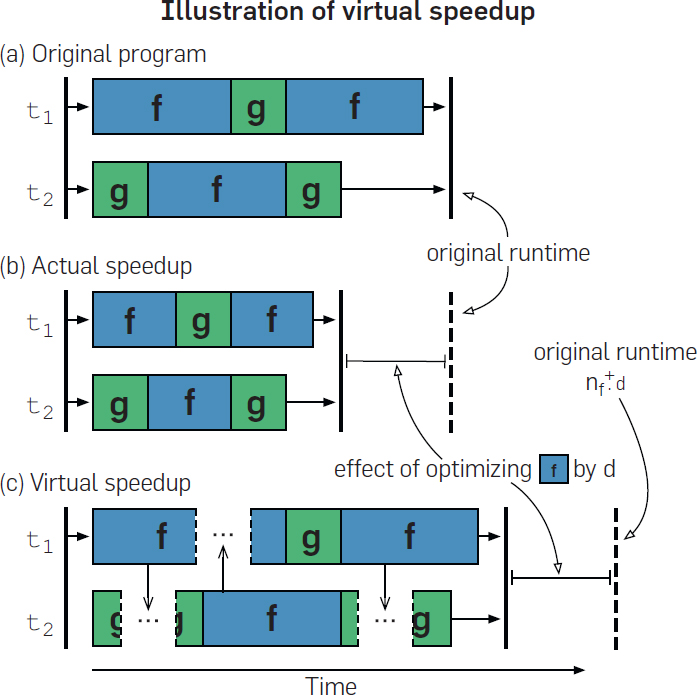
\includegraphics[width=0.4\textwidth]{images/virtual-speedup.jpg}
\end{center}

The tool provides some graphs of potential program speedup. From the recorded presentation, it might look something like the diagram below, where the boxes on the right correspond to different theoretical actions in the application being examined:

\begin{center}
	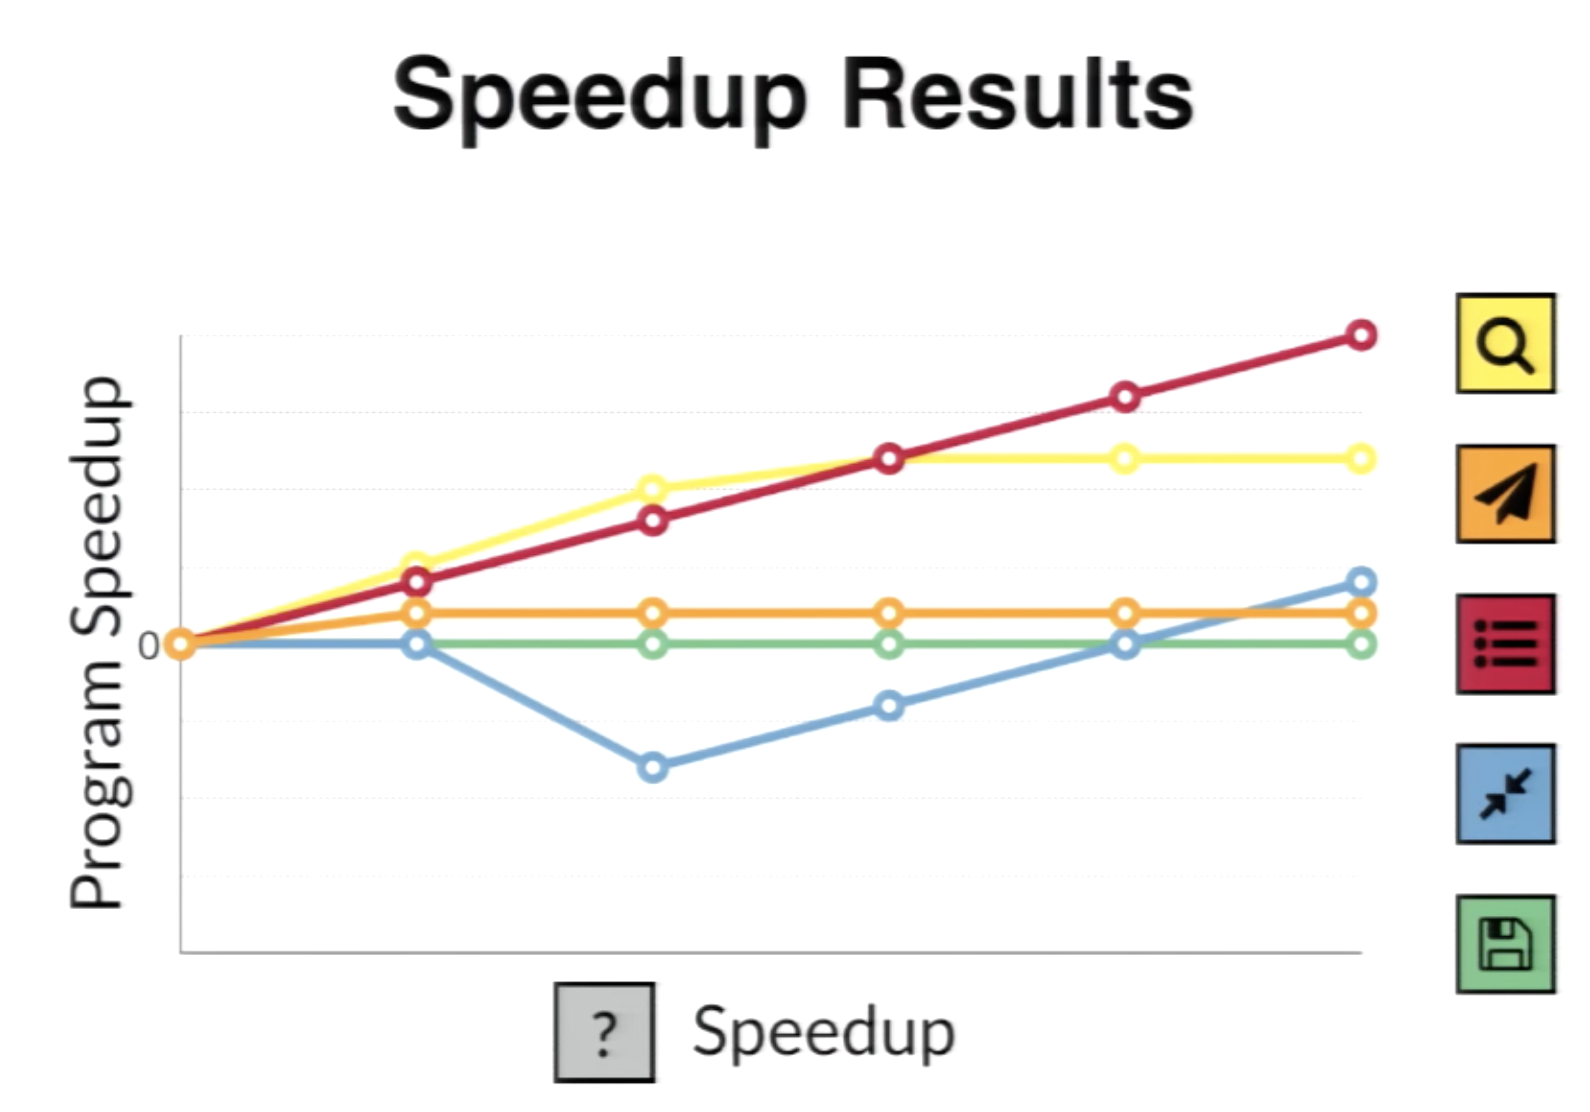
\includegraphics[width=0.4\textwidth]{images/coz-speedup-graph.png}
\end{center}

This pretend application shows all the possible outcomes, from continuous linear speedup, to speedup capped at some point, to no effect, and finally to where optimizing something makes the overall program runtime worse. 

It's easy to imagine scenarios corresponding to each of those. If we're computing the n-body problem, anything that improves the calculation of forces will certainly make things better. And it's easy to imagine that sometimes optimizing a part of the program does not improve anything because that code is not on the critical path. We can also easily imagine that improving something works up to a point where it ceases to be the limiting factor. But making things worse? We already covered that idea: speeding up a thread may increase lock contention or add something to the critical path. At some point, things may recover and be a net benefit.

It is important to remember that just because hypothetically speeding up a particular part of the program would be beneficial, doesn't mean that it's possible to speed up that part. And almost certainly not possible to do so to an arbitrary degree. We still have to make an assessment of what optimizations we can make and how difficult it would be to actually realize those improvements.

Once we've made a change to the program, then it's time to run an experiment again with the new baseline to see what else we can do.

The paper has a table summarizing the optimizations they applied to a few different programs, which seems to support the idea that the tool can be used effectively to get a meaningful speedup with relatively few lines of code~\cite{coz}:
\begin{center}
	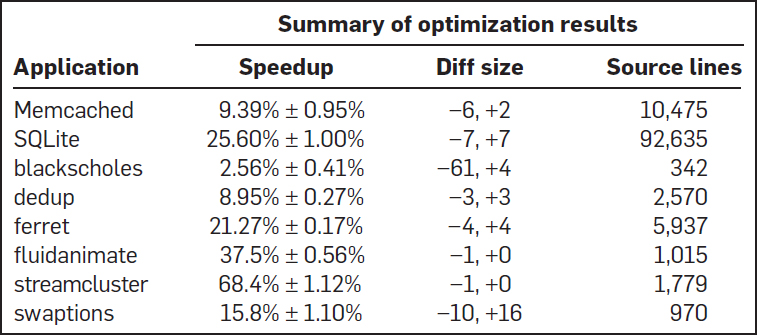
\includegraphics[width=0.6\textwidth]{images/coz-speedup.jpg}
\end{center}

There are potentially some limitations to this, of course. Putting pauses in the execution of the code can work when the execution of the program is all on the same machine and we have control over all the threads; it would need some meaningful extension to work for a distributed system where coordinating things across many servers would be needed.

Using some benchmarking workload, the authors estimate a 17.6\% overhead for this tool, which is broken down into 2.6\% for startup debug information collection, sampling at 4.8\%, and 10.2\% is the delay that's caused by slowing down other threads to create a virtual speedup~\cite{coz}.

If you'd like to see some more details of the tool, you can see the author presentation at the ACM symposium here: \url{https://www.youtube.com/watch?v=jE0V-p1odPg}

\section*{Memory Profiling}

Thus far we have focused on CPU profiling. Other kinds of profiling got some mention, but they're not the only kind of profiling we can do. Memory profiling is also a thing, and specifically we're going to focus on heap profiling.

During Rustification, we dropped a bunch of valgrind content. Valgrind is a memory error and leak detection toolset that is invaluable when programming in \CPP. (In brief: valgrind is a just-in-time engine that reinterprets machine code and instruments it to find sketchy things.) In particular, the memory leaks that valgrind's memcheck tool detects are, for the most part, not possible in Rust unless you try pretty hard\footnote{You can still create cycles in refcounted objects or call \texttt{std::mem::forget} or etc.}---the friendly compiler protects you against them by automatically dropping things.

We're going to look at two kinds of memory profiling here, both part of valgrind. They can both occur in Rust, but it looks like the more common kind is when a lot of memory is allocated and then freed. More completely: ``places that cause excessive numbers of allocations; leaks; unused and under-used allocations; short-lived allocations; and allocations with inefficient data layouts''. valgrind's DHAT tool~\cite[Chapter~10]{valgrind} detects these.

The second kind of memory profiling addresses memory that memcheck reports as ``Still Reachable''. That is, things that remained allocated and still had pointers to them, but were not properly deallocated. Right, we care about them too, and for that we also want to do heap profiling. If we don't look after those things, we're just using more and more memory over time. That likely means more paging and the potential for running out of heap space altogether. Again, the memory isn't really lost, because we could free it.

\subsection*{DHAT}
DHAT tracks allocation points and what happens to them over a program's execution. An allocation point is a point in the program which allocates memory; in C that would be \texttt{malloc}. In Rust there are a bunch of ways to allocate memory, one being \texttt{Box::new}. It aggregates allocation points according to the program stack. Let's first look at a leaf node from the documentation.

\begin{verbatim}
AP 1.1.1.1/2 {
  Total:     31,460,928 bytes (2.32%, 1,565.9/Minstr) in 262,171 blocks (4.41%, 13.05/Minstr), 
     avg size 120 bytes, avg lifetime 986,406,885.05 instrs (4.91% of program duration)
  Max:       16,779,136 bytes in 65,543 blocks, avg size 256 bytes
  At t-gmax: 0 bytes (0%) in 0 blocks (0%), avg size 0 bytes
  At t-end:  0 bytes (0%) in 0 blocks (0%), avg size 0 bytes
  Reads:     5,964,704 bytes (0.11%, 296.88/Minstr), 0.19/byte
  Writes:    10,487,200 bytes (0.51%, 521.98/Minstr), 0.33/byte
  Allocated at {
    ^1: 0x95CACC9: alloc (alloc.rs:72)
      [omitted]
    ^7: 0x95CACC9: parse_token_trees_until_close_delim (tokentrees.rs:27)
    ^8: 0x95CACC9: syntax::parse::lexer::tokentrees::<impl syntax::parse::lexer::
                          StringReader<'a>>::parse_token_tree (tokentrees.rs:81)
    ^9: 0x95CAC39: parse_token_trees_until_close_delim (tokentrees.rs:26)
    ^10: 0x95CAC39: syntax::parse::lexer::tokentrees::<impl syntax::parse::lexer::
                          StringReader<'a>>::parse_token_tree (tokentrees.rs:81)
    #11: 0x95CAC39: parse_token_trees_until_close_delim (tokentrees.rs:26)
    #12: 0x95CAC39: syntax::parse::lexer::tokentrees::<impl syntax::parse::lexer::
                          StringReader<'a>>::parse_token_tree (tokentrees.rs:81)
  }
}
\end{verbatim}

We can see the program point corresponding to this allocation: line 81 of \texttt{tokentrees.rs}.
Furthermore, the most bytes alive at once from this site was 16,779,136: that was 65,543 instances of the
memory allocated here, almost all 256-byte blocks. In total, this allocation site was executed
262,171 times, accounting for 31,460,928 bytes. This information can tell us how important this
allocation site is compared to the entire execution we're inspecting. We can also see how long-lived
the blocks are: on average, a block allocated here lives 4.91\% of the program duration. If instead of
4.91\% we had 0.004\% and a large total, then the allocation point would be excessively transient and perhaps
a good candidate for pooling allocations.

The Reads and Writes lines tell us how often the allocated memory is actually used. In this case,
19\% of the bytes allocated here are ever read, and 33\% are written to. That seems like not many, but if it's something
like a vector that grows, you may not be able to do anything about that. This, however, doesn't look like a vector---you
could check it by looking at the code.

You might also get a super-useful Accesses line if all of the blocks allocated at a site are the same size.
That line tells you how many times each byte in the block was accessed. Zeros, written as dashes (-), are
parts of the block that are never accessed, useful for finding data alignment holes (and hence potential
inefficiencies).

\paragraph{Parents.} Going up the tree, DHAT tells you about all of the allocation points that share a call-stack
prefix. (The \verb+^+ before the number indicates that the line is copied from the parent; a \# indicates that the line is unique to
that node.)

A sibling of the example above would diverge at the call on line 10, not calling
\texttt{parse\_token\_trees\_until\_close\_delim} from line 81 of \texttt{tokentrees.rs}. At the parent, DHAT
reports results for that node and all of its children.

\subsection*{\st{Memory Profiling} Return to Asgard}
JZ generally found a way to talk about Valgrind in previous courses. But now, we're going to use its Massif tool. This is, obviously, a joke on ``massive'', combined with the name Sif, a Norse goddess associated with the earth (and in the Marvel movies, Shieldmaiden to Thor).

So what does Massif do? It will tell you about how much heap memory your program is using, and also how the situation got to be that way. So let's start with the example program from the documentation, badly translated by yours truly to non-idiomatic Rust~\cite{massif}:


\begin{lstlisting}[language=Rust]
fn g() {
    let a = Vec::<u8>::with_capacity(4000);
    std::mem::forget(a)
}

fn f() {
    let a = Vec::<u8>::with_capacity(2000);
    std::mem::forget(a);
    g()
}

fn main() {

    let mut a = Vec::with_capacity(10);
    for _i in 0..10 {
	a.push(Box::new([0;1000]))
    }
    f();
    g();
}
\end{lstlisting}


After we compile, run the command:
{\scriptsize
\begin{verbatim}
plam@amqui ~/c/p/l/l/L/alloc> valgrind --tool=massif target/debug/alloc
==406569== Massif, a heap profiler
==406569== Copyright (C) 2003-2017, and GNU GPL'd, by Nicholas Nethercote
==406569== Using Valgrind-3.16.1 and LibVEX; rerun with -h for copyright info
==406569== Command: target/debug/alloc
==406569== 
==406569== 
\end{verbatim}
}

Doesn't that look useful?! What happened? Your program executed slowly, as is always the case with any of the Valgrind toolset, but you don't get summary data on the console like we did with Valgrind or helgrind or cachegrind. Weird. What we got instead was the file \texttt{massif.out.406569} (matches the PID of whatever we ran). This file, which you can open up in your favourite text editor, is not especially human readable, but it's not incomprehensible like the output from cachegrind (``Aha, a 1 in column 4 of line 2857. That's what's killing our performance!''). There is an associated tool for summarizing and interpreting this data in a much nicer way: \texttt{ms\_print}, which has nothing whatsoever to do with Microsoft. Promise.

If we look at the output there (hint: pipe the output to \texttt{less} or something, otherwise you get a huge amount of data thrown at the console), it looks much more user friendly.

{\scriptsize
\begin{verbatim}
    KB
78.57^                                                                       #
     |                                                                       #
     |                                                                       #
     |                                                                       #
     |                                                                       #
     |                                                                       #
     |                                                                       #
     |                                                                       #
     |                                                                       #
     |                                                                       #
     |                                                                       #
     |                                                                      :#
     |                                                                     @:#
     |                                                                    :@:#
     |                                                                    :@:#
     |                                                                   ::@:#
     |                                                                  :::@:#
     |                                                                  :::@:#
     |                                                                 ::::@:#
     |                                                                :::::@:#
   0 +----------------------------------------------------------------------->ki
     0                                                                   474.1
\end{verbatim}
}

Now wait a minute. This bar graph might be user friendly but it's not exactly what I'd call\ldots useful, is it? For a long time, nothing happens, then\ldots kaboom! According to the docs, what actually happened here is, we gave in a trivial program where most of the CPU time was spent doing the setup and loading and everything, and the trivial program ran for only a short period of time, right at the end. So for a relatively short program we should tell Massif to care more about the bytes than the CPU cycles, with the \verb+--time-unit=B+ option. Let's try that.

{\scriptsize
\begin{verbatim}
    KB
78.57^                                                ##                      
     |                                                # :::                   
     |                                                # :  ::                 
     |                                                # :  : ::               
     |                                       :::::::::# :  : : :::            
     |                                       :        # :  : : :  ::          
     |                                       :        # :  : : :  : ::        
     |                                       :        # :  : : :  : : :::     
     |                              ::::::::::        # :  : : :  : : :  ::   
     |                              :        :        # :  : : :  : : :  : :: 
     |                         ::::::        :        # :  : : :  : : :  : : @
     |                       :::    :        :        # :  : : :  : : :  : : @
     |                    @@@: :    :        :        # :  : : :  : : :  : : @
     |                  ::@  : :    :        :        # :  : : :  : : :  : : @
     |                ::: @  : :    :        :        # :  : : :  : : :  : : @
     |             :::: : @  : :    :        :        # :  : : :  : : :  : : @
     |           :::  : : @  : :    :        :        # :  : : :  : : :  : : @
     |         ::: :  : : @  : :    :        :        # :  : : :  : : :  : : @
     |      :::: : :  : : @  : :    :        :        # :  : : :  : : :  : : @
     |    :::  : : :  : : @  : :    :        :        # :  : : :  : : :  : : @
   0 +----------------------------------------------------------------------->KB
     0                                                                   121.6
\end{verbatim}
}

Neat. Now we're getting somewhere. We can see (from the text below the graph) that 48 snapshots were taken. It will take snapshots whenever there are appropriate allocation and deallocation statements, up to a configurable maximum, and for a long running program, toss some old data if necessary. Let's look in the documentation to see what the symbols mean (they're not just to look pretty). So, from the docs~\cite{massif}:

\begin{itemize}
\item Most snapshots are normal (they have just basic information) They use the `:' characters.

\item Detailed snapshots are shown with `@' characters.  By default, every 10th snapshot is detailed.

\item There is at most one peak snapshot. The peak snapshot is a detailed snapshot, and records the point where memory consumption was greatest. The peak snapshot is represented in the graph by a bar consisting of `\#' characters.
\end{itemize}

As a caveat, the peak can be a bit inaccurate. Peaks are only recorded when a deallocation happens. This just avoids wasting time recording a peak and then overwriting it; if you are allocating a bunch of blocks in succession (e.g. a bunch of structs that have a buffer) then you would constantly be overwriting the peak over and over again. Also, there's some loss of accuracy to speed things up. Well, okay.

So let's look at the snapshots. We'll start with the normal ones. Here are the first 5, numbers 0 through 4:

{\scriptsize
\begin{verbatim}
--------------------------------------------------------------------------------
  n        time(B)         total(B)   useful-heap(B) extra-heap(B)    stacks(B)
--------------------------------------------------------------------------------
  0              0                0                0             0            0
  1            488              488              472            16            0
  2            624              624              592            32            0
  3          1,656            1,656            1,616            40            0
  4          1,768            1,768            1,736            32            0
\end{verbatim}
}

The columns are pretty much self explanatory, with a couple exceptions. The time(B) column corresponds to time measured in allocations thanks to our choice of the time unit at the command line. The extra-heap(B) represents internal fragmentation\footnote{Remember from operating systems: if the user asked for some $n$ bytes where $n$ is not a nice multiple the returned block may be ``rounded up''. So a request for 1000 bytes is bumped up to 1016 bytes in this example. The extra space is ``wasted'' but it's nicer than having a whole bunch of little tiny useless fragments of the heap to be managed.} in the blocks we received. The stacks column shows as zero because by default, Massif doesn't look at the stack. It's a heap profiler, remember?

Number 5 is a ``detailed'' snapshot, so I've separated it out, and reproduced the headers there to make this a little easier to remember what they are.

{
\begin{verbatim}
--------------------------------------------------------------------------------
  n        time(B)         total(B)   useful-heap(B) extra-heap(B)    stacks(B)
--------------------------------------------------------------------------------
  5          1,768            1,768            1,736            32            0
98.19% (1,736B) (heap allocation functions) malloc/new/new[], --alloc-fns, etc.
->57.92% (1,024B) 0x492509B: _IO_file_doallocate (filedoalloc.c:101)
... etc
\end{verbatim}
}

So the additional information we got here is a reflection of where our heap allocations took place. Thus far, all the allocations are associated with the runtime library and {\tt lang\_start}, so not that useful to us.

Then let's look at the peak snapshot (again, trimmed significantly to call out the first thing we need to see here):

{
\begin{verbatim}
--------------------------------------------------------------------------------
  n        time(B)         total(B)   useful-heap(B) extra-heap(B)    stacks(B)
--------------------------------------------------------------------------------
 31         84,072           80,456           80,285           171            0
99.79% (80,285B) (heap allocation functions) malloc/new/new[], --alloc-fns, etc.
->99.53% (80,080B) 0x10F97B: alloc::alloc::alloc (alloc.rs:81)
| ->49.82% (40,080B) 0x10F771: <alloc::alloc::Global as core::alloc::Alloc>::alloc (alloc.rs:169)
| | ->49.72% (40,000B) 0x10D90D: alloc::raw_vec::RawVec<T,A>::allocate_in (raw_vec.rs:88)
| | | ->49.72% (40,000B) 0x10D744: alloc::raw_vec::RawVec<T>::with_capacity (raw_vec.rs:140)
| | |   ->49.72% (40,000B) 0x10C412: alloc::vec::Vec<T>::with_capacity (vec.rs:355)
| | |     ->39.77% (32,000B) 0x10FCF2: alloc::g (main.rs:2)
| | |     | ->19.89% (16,000B) 0x10FD5F: alloc::f (main.rs:9)
\end{verbatim}
}

Massif has found all the allocations in this program and distilled them down to a tree structure that traces the path through which all of these various memory allocations occurred. So not just where the \texttt{malloc} call happened, but also how we got there. With lots of Rust helper functions as well.

If I ask valgrind what it thinks of this program, it says:

{\scriptsize
\begin{verbatim}
plam@amqui ~/c/p/l/l/L/alloc> valgrind target/debug/alloc
==406822== Memcheck, a memory error detector
==406822== Copyright (C) 2002-2017, and GNU GPL'd, by Julian Seward et al.
==406822== Using Valgrind-3.16.1 and LibVEX; rerun with -h for copyright info
==406822== Command: target/debug/alloc
==406822== 
==406822== 
==406822== HEAP SUMMARY:
==406822==     in use at exit: 40,000 bytes in 3 blocks
==406822==   total heap usage: 25 allocs, 22 frees, 82,177 bytes allocated
==406822== 
==406822== LEAK SUMMARY:
==406822==    definitely lost: 40,000 bytes in 3 blocks
==406822==    indirectly lost: 0 bytes in 0 blocks
==406822==      possibly lost: 0 bytes in 0 blocks
==406822==    still reachable: 0 bytes in 0 blocks
==406822==         suppressed: 0 bytes in 0 blocks
==406822== Rerun with --leak-check=full to see details of leaked memory
==406822== 
==406822== For lists of detected and suppressed errors, rerun with: -s
==406822== ERROR SUMMARY: 0 errors from 0 contexts (suppressed: 0 from 0)
\end{verbatim}
}

We used to say: ``So probably a good idea to run valgrind first and make it happy before we go into figuring out where heap blocks are going with Massif.'' Now, well, just use Rust and then DHAT. But Massif is still another tool at your disposal. Okay, what to do with the information from Massif, anyway? It should be pretty easy to act upon this information. Start with the peak snapshot (worst case scenario) and see where that takes you (if anywhere). You can probably identify some cases where memory is hanging around unnecessarily. 

Things to watch out for:
\begin{itemize}
\item memory usage climbing over a long period of time, perhaps slowly, but never really decreasing---memory is filling up somehow with some junk? 
\item large spikes in the graph---why so much allocation and deallocation in a short period?
\end{itemize}

Other cool things we can do with Massif~\cite{massif}:

\begin{itemize}
	\item Look into stack allocation (\verb+--stacks=yes+) option. This slows stuff down a lot, and not really necessary since we want to look at heap.
	\item Look at the children of a process (anything split off with \texttt{fork}) if desired.
	\item Check low level stuff: if we're doing something other than \texttt{malloc}, \texttt{calloc}, \texttt{new}, etc. and doing low level stuff like \texttt{mmap} or \texttt{brk} that is usually missed, but we can do profiling at page level (\verb+--pages-as-heap=yes+).
\end{itemize}

% which programs to live demo?
As is often the case, we have examined how the tool works on a trivial program. As a live demo, well, tune in and be surprised!
%let's see what happens when we take the program complexity up a little bit by (1) looking at the search program we saw in the earlier talk about valgrind; and (2) looking at the original (unmodified) paster.c file from assignment 1 (and then perhaps fixing it and going on). Depending on time available, we may look at some more complex programs.

\bibliographystyle{alphaurl}
\bibliography{459}


\end{document}
